
\documentclass[10pt,journal,compsoc]{IEEEtran}

% Some very useful LaTeX packages include:
% (uncomment the ones you want to load)


% *** MISC UTILITY PACKAGES ***
%
%\usepackage{ifpdf}
% Heiko Oberdiek's ifpdf.sty is very useful if you need conditional
% compilation based on whether the output is pdf or dvi.
% usage:
% \ifpdf
%   % pdf code
% \else
%   % dvi code
% \fi
% The latest version of ifpdf.sty can be obtained from:
% http://www.ctan.org/pkg/ifpdf
% Also, note that IEEEtran.cls V1.7 and later provides a builtin
% \ifCLASSINFOpdf conditional that works the same way.
% When switching from latex to pdflatex and vice-versa, the compiler may
% have to be run twice to clear warning/error messages.






% *** CITATION PACKAGES ***
%
\ifCLASSOPTIONcompsoc
  % IEEE Computer Society needs nocompress option
  % requires cite.sty v4.0 or later (November 2003)
  \usepackage[nocompress]{cite}
\else
  % normal IEEE
  \usepackage{cite}
\fi
% cite.sty was written by Donald Arseneau
% V1.6 and later of IEEEtran pre-defines the format of the cite.sty package
% \cite{} output to follow that of the IEEE. Loading the cite package will
% result in citation numbers being automatically sorted and properly
% "compressed/ranged". e.g., [1], [9], [2], [7], [5], [6] without using
% cite.sty will become [1], [2], [5]--[7], [9] using cite.sty. cite.sty's
% \cite will automatically add leading space, if needed. Use cite.sty's
% noadjust option (cite.sty V3.8 and later) if you want to turn this off
% such as if a citation ever needs to be enclosed in parenthesis.
% cite.sty is already installed on most LaTeX systems. Be sure and use
% version 5.0 (2009-03-20) and later if using hyperref.sty.
% The latest version can be obtained at:
% http://www.ctan.org/pkg/cite
% The documentation is contained in the cite.sty file itself.
%
% Note that some packages require special options to format as the Computer
% Society requires. In particular, Computer Society  papers do not use
% compressed citation ranges as is done in typical IEEE papers
% (e.g., [1]-[4]). Instead, they list every citation separately in order
% (e.g., [1], [2], [3], [4]). To get the latter we need to load the cite
% package with the nocompress option which is supported by cite.sty v4.0
% and later. Note also the use of a CLASSOPTION conditional provided by
% IEEEtran.cls V1.7 and later.





% *** GRAPHICS RELATED PACKAGES ***
%
\ifCLASSINFOpdf
  % \usepackage[pdftex]{graphicx}
  % declare the path(s) where your graphic files are
  % \graphicspath{{../pdf/}{../jpeg/}}
  % and their extensions so you won't have to specify these with
  % every instance of \includegraphics
  % \DeclareGraphicsExtensions{.pdf,.jpeg,.png}
\else
  % or other class option (dvipsone, dvipdf, if not using dvips). graphicx
  % will default to the driver specified in the system graphics.cfg if no
  % driver is specified.
  % \usepackage[dvips]{graphicx}
  % declare the path(s) where your graphic files are
  % \graphicspath{{../eps/}}
  % and their extensions so you won't have to specify these with
  % every instance of \includegraphics
  % \DeclareGraphicsExtensions{.eps}
\fi
% graphicx was written by David Carlisle and Sebastian Rahtz. It is
% required if you want graphics, photos, etc. graphicx.sty is already
% installed on most LaTeX systems. The latest version and documentation
% can be obtained at: 
% http://www.ctan.org/pkg/graphicx
% Another good source of documentation is "Using Imported Graphics in
% LaTeX2e" by Keith Reckdahl which can be found at:
% http://www.ctan.org/pkg/epslatex
%
% latex, and pdflatex in dvi mode, support graphics in encapsulated
% postscript (.eps) format. pdflatex in pdf mode supports graphics
% in .pdf, .jpeg, .png and .mps (metapost) formats. Users should ensure
% that all non-photo figures use a vector format (.eps, .pdf, .mps) and
% not a bitmapped formats (.jpeg, .png). The IEEE frowns on bitmapped formats
% which can result in "jaggedy"/blurry rendering of lines and letters as
% well as large increases in file sizes.
%
% You can find documentation about the pdfTeX application at:
% http://www.tug.org/applications/pdftex






% *** MATH PACKAGES ***
%
%\usepackage{amsmath}
% A popular package from the American Mathematical Society that provides
% many useful and powerful commands for dealing with mathematics.
%
% Note that the amsmath package sets \interdisplaylinepenalty to 10000
% thus preventing page breaks from occurring within multiline equations. Use:
%\interdisplaylinepenalty=2500
% after loading amsmath to restore such page breaks as IEEEtran.cls normally
% does. amsmath.sty is already installed on most LaTeX systems. The latest
% version and documentation can be obtained at:
% http://www.ctan.org/pkg/amsmath





% *** SPECIALIZED LIST PACKAGES ***
%
%\usepackage{algorithmic}
% algorithmic.sty was written by Peter Williams and Rogerio Brito.
% This package provides an algorithmic environment fo describing algorithms.
% You can use the algorithmic environment in-text or within a figure
% environment to provide for a floating algorithm. Do NOT use the algorithm
% floating environment provided by algorithm.sty (by the same authors) or
% algorithm2e.sty (by Christophe Fiorio) as the IEEE does not use dedicated
% algorithm float types and packages that provide these will not provide
% correct IEEE style captions. The latest version and documentation of
% algorithmic.sty can be obtained at:
% http://www.ctan.org/pkg/algorithms
% Also of interest may be the (relatively newer and more customizable)
% algorithmicx.sty package by Szasz Janos:
% http://www.ctan.org/pkg/algorithmicx




% *** ALIGNMENT PACKAGES ***
%
%\usepackage{array}
% Frank Mittelbach's and David Carlisle's array.sty patches and improves
% the standard LaTeX2e array and tabular environments to provide better
% appearance and additional user controls. As the default LaTeX2e table
% generation code is lacking to the point of almost being broken with
% respect to the quality of the end results, all users are strongly
% advised to use an enhanced (at the very least that provided by array.sty)
% set of table tools. array.sty is already installed on most systems. The
% latest version and documentation can be obtained at:
% http://www.ctan.org/pkg/array


% IEEEtran contains the IEEEeqnarray family of commands that can be used to
% generate multiline equations as well as matrices, tables, etc., of high
% quality.




% *** SUBFIGURE PACKAGES ***
%\ifCLASSOPTIONcompsoc
%  \usepackage[caption=false,font=footnotesize,labelfont=sf,textfont=sf]{subfig}
%\else
%  \usepackage[caption=false,font=footnotesize]{subfig}
%\fi
% subfig.sty, written by Steven Douglas Cochran, is the modern replacement
% for subfigure.sty, the latter of which is no longer maintained and is
% incompatible with some LaTeX packages including fixltx2e. However,
% subfig.sty requires and automatically loads Axel Sommerfeldt's caption.sty
% which will override IEEEtran.cls' handling of captions and this will result
% in non-IEEE style figure/table captions. To prevent this problem, be sure
% and invoke subfig.sty's "caption=false" package option (available since
% subfig.sty version 1.3, 2005/06/28) as this is will preserve IEEEtran.cls
% handling of captions.
% Note that the Computer Society format requires a sans serif font rather
% than the serif font used in traditional IEEE formatting and thus the need
% to invoke different subfig.sty package options depending on whether
% compsoc mode has been enabled.
%
% The latest version and documentation of subfig.sty can be obtained at:
% http://www.ctan.org/pkg/subfig




% *** FLOAT PACKAGES ***
%
%\usepackage{fixltx2e}
% fixltx2e, the successor to the earlier fix2col.sty, was written by
% Frank Mittelbach and David Carlisle. This package corrects a few problems
% in the LaTeX2e kernel, the most notable of which is that in current
% LaTeX2e releases, the ordering of single and double column floats is not
% guaranteed to be preserved. Thus, an unpatched LaTeX2e can allow a
% single column figure to be placed prior to an earlier double column
% figure.
% Be aware that LaTeX2e kernels dated 2015 and later have fixltx2e.sty's
% corrections already built into the system in which case a warning will
% be issued if an attempt is made to load fixltx2e.sty as it is no longer
% needed.
% The latest version and documentation can be found at:
% http://www.ctan.org/pkg/fixltx2e


%\usepackage{stfloats}
% stfloats.sty was written by Sigitas Tolusis. This package gives LaTeX2e
% the ability to do double column floats at the bottom of the page as well
% as the top. (e.g., "\begin{figure*}[!b]" is not normally possible in
% LaTeX2e). It also provides a command:
%\fnbelowfloat
% to enable the placement of footnotes below bottom floats (the standard
% LaTeX2e kernel puts them above bottom floats). This is an invasive package
% which rewrites many portions of the LaTeX2e float routines. It may not work
% with other packages that modify the LaTeX2e float routines. The latest
% version and documentation can be obtained at:
% http://www.ctan.org/pkg/stfloats
% Do not use the stfloats baselinefloat ability as the IEEE does not allow
% \baselineskip to stretch. Authors submitting work to the IEEE should note
% that the IEEE rarely uses double column equations and that authors should try
% to avoid such use. Do not be tempted to use the cuted.sty or midfloat.sty
% packages (also by Sigitas Tolusis) as the IEEE does not format its papers in
% such ways.
% Do not attempt to use stfloats with fixltx2e as they are incompatible.
% Instead, use Morten Hogholm'a dblfloatfix which combines the features
% of both fixltx2e and stfloats:
%
% \usepackage{dblfloatfix}
% The latest version can be found at:
% http://www.ctan.org/pkg/dblfloatfix




%\ifCLASSOPTIONcaptionsoff
%  \usepackage[nomarkers]{endfloat}
% \let\MYoriglatexcaption\caption
% \renewcommand{\caption}[2][\relax]{\MYoriglatexcaption[#2]{#2}}
%\fi
% endfloat.sty was written by James Darrell McCauley, Jeff Goldberg and 
% Axel Sommerfeldt. This package may be useful when used in conjunction with 
% IEEEtran.cls'  captionsoff option. Some IEEE journals/societies require that
% submissions have lists of figures/tables at the end of the paper and that
% figures/tables without any captions are placed on a page by themselves at
% the end of the document. If needed, the draftcls IEEEtran class option or
% \CLASSINPUTbaselinestretch interface can be used to increase the line
% spacing as well. Be sure and use the nomarkers option of endfloat to
% prevent endfloat from "marking" where the figures would have been placed
% in the text. The two hack lines of code above are a slight modification of
% that suggested by in the endfloat docs (section 8.4.1) to ensure that
% the full captions always appear in the list of figures/tables - even if
% the user used the short optional argument of \caption[]{}.
% IEEE papers do not typically make use of \caption[]'s optional argument,
% so this should not be an issue. A similar trick can be used to disable
% captions of packages such as subfig.sty that lack options to turn off
% the subcaptions:
% For subfig.sty:
% \let\MYorigsubfloat\subfloat
% \renewcommand{\subfloat}[2][\relax]{\MYorigsubfloat[]{#2}}
% However, the above trick will not work if both optional arguments of
% the \subfloat command are used. Furthermore, there needs to be a
% description of each subfigure *somewhere* and endfloat does not add
% subfigure captions to its list of figures. Thus, the best approach is to
% avoid the use of subfigure captions (many IEEE journals avoid them anyway)
% and instead reference/explain all the subfigures within the main caption.
% The latest version of endfloat.sty and its documentation can obtained at:
% http://www.ctan.org/pkg/endfloat
%
% The IEEEtran \ifCLASSOPTIONcaptionsoff conditional can also be used
% later in the document, say, to conditionally put the References on a 
% page by themselves.




% *** PDF, URL AND HYPERLINK PACKAGES ***
%
%\usepackage{url}
% url.sty was written by Donald Arseneau. It provides better support for
% handling and breaking URLs. url.sty is already installed on most LaTeX
% systems. The latest version and documentation can be obtained at:
% http://www.ctan.org/pkg/url
% Basically, \url{my_url_here}.





% *** Do not adjust lengths that control margins, column widths, etc. ***
% *** Do not use packages that alter fonts (such as pslatex).         ***
% There should be no need to do such things with IEEEtran.cls V1.6 and later.
% (Unless specifically asked to do so by the journal or conference you plan
% to submit to, of course. )
\usepackage{cite}
\usepackage{amsmath,amssymb,amsfonts}
\usepackage{algorithmic}
\usepackage{graphicx}
\usepackage{textcomp}

% correct bad hyphenation here
\hyphenation{op-tical net-works semi-conduc-tor}


\begin{document}
%
% paper title
% Titles are generally capitalized except for words such as a, an, and, as,
% at, but, by, for, in, nor, of, on, or, the, to and up, which are usually
% not capitalized unless they are the first or last word of the title.
% Linebreaks \\ can be used within to get better formatting as desired.
% Do not put math or special symbols in the title.
	%\title{Bare Demo of IEEEtran.cls for\\ IEEE Computer Society Journals}
%
\title{Overtaking Uncertainty with Evolutionary Drivers for TORCS: Combining BLX-$\alpha$ Operator and Grand Prix Selection}

\author{Mohammed~Salem, Antonio~M.~Mora, and~Juan~J.~Merelo% <-this % stops a space
\IEEEcompsocitemizethanks{\IEEEcompsocthanksitem M. Salem was with the Department of Computer Sciences, University of Mascara, Algeria.\protect\\
% note need leading \protect in front of \\ to get a newline within \thanks as
% \\ is fragile and will error, could use \hfil\break instead.
E-mail: salem@univ-mascara.dz
\IEEEcompsocthanksitem A~M.~Mora was with the Department of Signal Theory, Telematics and Communications, ETSIIT-CITIC, University of Granada, Spain.\protect\\
Email: amorag@ugr.es
\IEEEcompsocthanksitem J~J.~Merelo was with the Department of Computer Architecture and Computer Technology. University of Granada, Spain.\protect\\
Email: jmerelo@geneura.ugr.es
}% <-this % stops an unwanted space
\thanks{Manuscript received December XX, 2019; revised XXXX, 2020.}}

% note the % following the last \IEEEmembership and also \thanks - 
% these prevent an unwanted space from occurring between the last author name
% and the end of the author line. i.e., if you had this:
% 
% \author{....lastname \thanks{...} \thanks{...} }
%                     ^------------^------------^----Do not want these spaces!
%
% a space would be appended to the last name and could cause every name on that
% line to be shifted left slightly. This is one of those "LaTeX things". For
% instance, "\textbf{A} \textbf{B}" will typeset as "A B" not "AB". To get
% "AB" then you have to do: "\textbf{A}\textbf{B}"
% \thanks is no different in this regard, so shield the last } of each \thanks
% that ends a line with a % and do not let a space in before the next \thanks.
% Spaces after \IEEEmembership other than the last one are OK (and needed) as
% you are supposed to have spaces between the names. For what it is worth,
% this is a minor point as most people would not even notice if the said evil
% space somehow managed to creep in.



% The paper headers
\markboth{Journal of \LaTeX\ Class Files,~Vol.~14, No.~8, August~2015}%
{Shell \MakeLowercase{\textit{et al.}}: Bare Demo of IEEEtran.cls for Computer Society Journals}
% The only time the second header will appear is for the odd numbered pages
% after the title page when using the twoside option.
% 
% *** Note that you probably will NOT want to include the author's ***
% *** name in the headers of peer review papers.                   ***
% You can use \ifCLASSOPTIONpeerreview for conditional compilation here if
% you desire.



% The publisher's ID mark at the bottom of the page is less important with
% Computer Society journal papers as those publications place the marks
% outside of the main text columns and, therefore, unlike regular IEEE
% journals, the available text space is not reduced by their presence.
% If you want to put a publisher's ID mark on the page you can do it like
% this:
%\IEEEpubid{0000--0000/00\$00.00~\copyright~2015 IEEE}
% or like this to get the Computer Society new two part style.
%\IEEEpubid{\makebox[\columnwidth]{\hfill 0000--0000/00/\$00.00~\copyright~2015 IEEE}%
%\hspace{\columnsep}\makebox[\columnwidth]{Published by the IEEE Computer Society\hfill}}
% Remember, if you use this you must call \IEEEpubidadjcol in the second
% column for its text to clear the IEEEpubid mark (Computer Society jorunal
% papers don't need this extra clearance.)



% use for special paper notices
%\IEEEspecialpapernotice{(Invited Paper)}



% for Computer Society papers, we must declare the abstract and index terms
% PRIOR to the title within the \IEEEtitleabstractindextext IEEEtran
% command as these need to go into the title area created by \maketitle.
% As a general rule, do not put math, special symbols or citations
% in the abstract or keywords.
\IEEEtitleabstractindextext{%
\begin{abstract}
Uncertainty, also called \textit{noise}, is one of the principal issues to address in the construction of algorithms to improve autonomous drivers. This effect means that a specific controller can be evaluated as very good or on the contrary as very bad, depending on `external' conditions, such as the behaviour of the competitors (other controllers) in the race, or the track status, for instance.
The evolutionary fuzzy-based driver proposed in previous works by the authors also suffered from that problem. It was composed of two fuzzy subcontrollers: one for selecting the best wheel steering angle and another to set the car target speed at the next simulation tick. Both where refined by applying a genetic algorithm on their parameterization.
Thus, in this paper we propose the improvement of our previous controller by means of two techniques. First, a Blend Crossover (\textit{BLX-$\alpha$}) operator has been applied during the search, in order to enhance diversity in the population of solutions. Together with this operator, a novel fitness-less selection mechanism has been considered: \textit{Grand Prix selection}. It is based on conducting a set of races involving some individuals (potential controllers) in order to select the winners as parents for the next generation.
The effectiveness of those mechanisms has been studied in several experiments, aiming to see the impact of each of them in the quality of the obtained controllers, as well as to determine the best configuration for an autonomous driver to win other existing controllers from the literature.
\end{abstract}

% Note that keywords are not normally used for peerreview papers.
\begin{IEEEkeywords}
Simulated Car Racing, TORCS, Fuzzy Controllers, Autonomous Drivers, Genetic Algorithms, Optimization, BLX-$\alpha$ Crossover, Grand Prix Selection, Uncertainty.
\end{IEEEkeywords}}


% make the title area
\maketitle


% To allow for easy dual compilation without having to reenter the
% abstract/keywords data, the \IEEEtitleabstractindextext text will
% not be used in maketitle, but will appear (i.e., to be "transported")
% here as \IEEEdisplaynontitleabstractindextext when the compsoc 
% or transmag modes are not selected <OR> if conference mode is selected 
% - because all conference papers position the abstract like regular
% papers do.
\IEEEdisplaynontitleabstractindextext
% \IEEEdisplaynontitleabstractindextext has no effect when using
% compsoc or transmag under a non-conference mode.



% For peer review papers, you can put extra information on the cover
% page as needed:
% \ifCLASSOPTIONpeerreview
% \begin{center} \bfseries EDICS Category: 3-BBND \end{center}
% \fi
%
% For peerreview papers, this IEEEtran command inserts a page break and
% creates the second title. It will be ignored for other modes.
\IEEEpeerreviewmaketitle



\IEEEraisesectionheading{\section{Introduction}\label{sec:introduction}}

% -------------- Comments this out since this is in other papers and
% off focus ----------------------------------------------------------

% Games are, in many cases, closed and controlled environments, mini or
% simulated worlds that allow you to test techniques that will then
% eventually be applied in real life, probably combined with other
% different technologies to tackle its complexity and variability. Car
% racing simulation includes many of the factors that are present in
% autonomous driving: tracks are very different and not known in
% advance, there are other vehicles present on the track, and the
% conditions change according to weather, and car deteriorates with
% damage. Car is also aware of this only through a set of limited
% sensors, and it will have to take a decision on speed and steering that is optimal in several different senses \cite{Autodriv2006}, including, depending on the context, the possibility of beating a set of opponents in a simulated race.

% Since testing different autonomous driving methodologies in real life is
% usually reserved to just a few big players, methodologies 
% as well as algorithms are usually tested in simulated environments;
% these simulated environments, at the same time, offer the incentive of
% competition among your system and others. In this paper, we will be
% using The Open Racing Car Simulator (TORCS) \cite{torcs4}, a very
% realistic racing simulator which offers a great testbed for the
% implementation and evaluation of autonomous drivers.  
% It has been used several times for the celebration of Artificial
% Intelligence (AI) competitions, where the aim is to create the best
% autonomous driver for racing
% \cite{SimulatedCarRacing-2008,SimulatedCarRacing-2010,manualTORCS}. Besides being able to test your car against other cars that have been published, it can be used as a standalone environment to optimize driving in a
% solo race. 

% Evolutionary Algorithms (EAs) \cite{EAs_Back96} have been frequently
% applied as a general-purpose optimization method in this area,
% generally combined with behavioural engines that rule different parts
% of the car
% \cite{CarRacing_Pelta09,SAES2012,Autopia2012}. These
% driving engines have included lately fuzzy controllers
% \cite{Guadarrama2008, LFAG, PerezEvolvingFuzzy09}. These controllers
% use fuzzy Logic \cite{Fuzzy2011}, a  technique that is quite suitable
% for defining this kind of autonomous agents, since they are in part
% inspired by the human reasoning when driving. A fuzzy controller works
% with linguistic variables, and will for instance turn {\em slightly}
% to the right when the next curve is {\em close}, but these controllers
% have to be designed to map properly inputs to desired outputs in
% particular situations. 
% --------------------------------------------------------------------



% -------------- This is also the same, but more to the point-------
% Need to rewrite anyway -------------------------------------------

% From the point of view of optimization, one of the main problems is
% that the environment is always going to change; this is correctly
% reflected in the simulator used, and it means that the score (and
% thus the ranking, if that's the eventual target) will always change,
% making selection of the {\em best} or {\em winning} controller
% probabilistic at best. This uncertainty is a challenge from two points
% of view: non optimal (non-winning) controllers might be selected just
% by chance, since they were assigned a score favored by that
% uncertainty, and, once they are selected, that might make the
% algorithm explore zones around some controllers that have been
% selected just casually, and leave others unexplored. For these two
% reasons, there are two challenges that we intend to approach in this
% paper: reduce uncertainty in the selection of the ``best'', and keep
% diversity high to not exploit just the areas around those individuals
% whose score might have been favored by chance at a certain point in
% the evolution process.
% --------------------------------------------------------------------

% % Antonio - Previous works
% Previously, the authors presented an approach combining two specialized fuzzy controllers, designed by hand, that were able to decide the car's proper steering angle and desired speed at every single point (or tick) during a race \cite{salem_evo17}. This driver was later improved \cite{salem_evo18} optimizing the parameters of their membership functions by means of a Genetic Algorithm
% \cite{GAs_Goldberg89}; this automated design improved manual one
% obtaining several controllers that were able to beat the initial
% hand-designed controller in a race, as well as other published
% controllers. Finally, the authors enhanced the controller in the last paper \cite{salem_cig2018} by means of the definition of new fitness functions. The selection of the best controller at the end of the evolution was based on a set of races among the best 4 solutions, getting a better driver than in previous studies.

% This proved that evolutionary algorithms were able to get the fuzzy
% controller parameters better than a hand-made design, but at the same
% time revealed several challenges. In general, evolutionary algorithms
% optimize the fitness function that is used; evolved fuzzy controllers
% (hereafter FCs) will be eventually as good as the fitness function allows. 
% But in this particular case we cannot use as fitness function the position
% obtained by the FC in every possible race on every possible track with
% every possible opponent, so we have to settle for a {\em surrogate} of
% the fitness in a very limited environment. First we opted for
% eliminating opponents and making evaluations in solo races; then we
% chose a particular track that combined straight segments as well as
% some curves and did not take too long to run, and eventually we had to
% decide what factors related to speed, damage and lap time were going
% to be effectively included in the final fitness function. 


% The two new techniques introduced in this paper, namely, \textit{Grand Prix selection} (GPS) and $BLX-\alpha$ crossover, try to improve on previous results by first relying less on the surrogacy of the fitness function
% to select the best individuals. The GPS will use a parameter-less fitness function to select a few individuals that will race against each other; racing will {\em smooth out} randomness in the fitness by putting them in a
% more real environment; racing cars against each other will offer a
% result that varies much less than simply comparing fitness. But, even
% so, uncertainty is present in the fitness and we should avoid
% excessive exploitation of the results. The $BLX-\alpha$ crossover we
% have introduced takes care of this aspect.

% With these methods we aim to obtain more reliable and competitive controllers and we will test them against some tough opponents, including a controller from the state of the art in Simulated Car Racing Competitions.

%The rest of the paper is organized as follows. Next we present the
%state of the art, to be followed by a description of the TORCS
%simulator \ref{sec:torcs}, the defined fuzzy controllers \ref{sec:subcontrollers} and a deep explanation of the Genetic Algorithm implemented and tested in this work in Section \ref{sec:GA_optimization}. 
%After it, the experiments conducted and the obtained results are described in Section \ref{sec:results}. Finally, conclusions and future lines of work will be presented in Section \ref{sec:conclusions}.


%%%%%%%%%%%%%%%%%%%%%%%%%%%%%%  STATE OF THE ART  %%%%%%%%%%%%%%%%%%%%%%%%%%%%%%
\section{State of the Art}
\label{sec:soa}


% We have to focus the state of the art in three different things
% 1. First and foremost, uncertainty in evolution, since it's in the
% title of the paper.
% 2. Second, alternative selection operators used in games, similar to
% the Grand Prix selection.
% 3. State of the art in TORCS since our last paper (CoG 2019)

% \cite{vrajitoru2019trajectory} maps the trajectory using the first lap and then optimizes it using an evolutionary algorithm.

%%%%%%%%%%%%%%%%%%%%%%%%%%%%%%  TORCS  %%%%%%%%%%%%%%%%%%%%%%%%%%%%%%

\section{The Open Racing Car Simulator}
\label{sec:torcs}

The framework in which this study has been conducted is TORCS \cite{torcs4}. It is an open source, multi-player, modular and portable racing simulator that allows users to compete against other computer-controlled opponents.
Its high degree of modularity and portability, together with the
realistic and real-time driving simulation, make it an ideal testbed
for artificial intelligence research, as stated in previous section.

Every car in TORCS includes  a large set of sensors \cite{manualTORCS},
whose values the car can use during a race, such as distances to track borders, to rivals, current fuel, current gear, position in the race, speed, or damage, among others. See Figure \ref{fig:torcs-sensors}.

\begin{figure}[!ht] 
	\begin{center}
		\includegraphics[scale=0.35]{fig/torcs-sensors}
		\caption {TORCS capture showing some of the sensors that the car includes.}
		\label{fig:torcs-sensors}
	\end{center}
	% Antonio - if we need space we can remove this image
\end{figure}


The sensor values are considered by any TORCS autonomous driver, or
{\em controller}, to manage the car using actuators \cite{manualTORCS}: the
steering wheel, the accelerator, the brake pedal and the gearbox.   


%*****************************  FUZZY CONTROLLER  ******************************

\section{Fuzzy sub-controllers}
\label{sec:subcontrollers}

% This section should probably be eliminated except. There's no part that's original. We should just summarize it in the next section, and make a reference to published papers - JJ

% We initially proposed a controller \cite{salem_evo17} with the same modular architecture as the simple TORCS driver; however, the target speed and
% steering angle are computed by means of two modular and specialized
% fuzzy sub-controllers, which consider five position sensors. This is
% the controller which will be improved by means of a GA in this
% work.

% The \textbf{fuzzy target speed sub-controller} aims to estimate the
% optimal target speed of the car, both in straight parts and curves of
% the track, taking into account two criteria: move as fast as possible
% and be safe. This estimation is based on two general cases: if the car
% is in a straight line, the target speed will take a maximum value
% (\textit{maxSpeed} km/h). However, if it is close to a curve, the
% controller will decrease the current speed to a value included in the
% interval \textit{[minSpeed, maxSpeed]} km/h. 

% This fuzzy controller has an output, the speed, and three input values (See Figure \ref{fig:torcs-sensors}):
% \begin{itemize}
% 	\item Front = Track\_9: front distance to the track border (angle 0\textdegree).  
% 	\item M5 = max (Track\_8, Track\_10): max distance to the track border in an angle of +5\textdegree and -5\textdegree with respect to Front.
% 	\item M10 = max (Track\_7, Track\_11): max distance to track border in an angle of +10\textdegree and -10\textdegree.
% \end{itemize}

% It is a Mamdani-based fuzzy system \cite{iancu2012} with three
% trapezoidal Membership Functions (MF) for every input variable. 
% %The description of these fuzzy inputs and output are represented in Table
% %\ref{tab:flouevar}. 
% In \cite{salem_evo18} the different sets of parameters which define the membership functions were improved using a Genetic Algorithm to obtain the best results.

% Moreover, the controller is based in a set of fuzzy rules, designed to
% maximize the car speed depending on the distance to the track
% border. These rules are \cite{salem_evo17}:
%  \begin{itemize}
%  {\small
%  	\item \texttt{IF Front is High THEN TargetSpeed is TS1}
%  	\item \texttt{IF Front is Medium THEN TargetSpeed is TS2}
%  	\item \texttt{IF Front is Low and M5 is High THEN TargetSpeed is TS3}
%  	\item \texttt{IF Front is Low and M5 is Medium THEN TargetSpeed is TS4}
%  	\item \texttt{IF Front is Low and M5 is Low and M10 is High THEN TargetSpeed is TS5}
%  	\item \texttt{IF Front is Low and M5 is Low and M10 is Medium THEN TargetSpeed is TS6}
%  	\item \texttt{IF Front is Low and M5 is Low and M10 is Low THEN TargetSpeed is TS7}\\
%  }
% %
% In addition, a crisp rule is added to obtain a maximum value of the target speed when the three input variables are as big as possible:\\
%  {\small	
%  \item \texttt{IF Front = MAXDISTSPEED or M5 = MAXDISTSPEED or M10 = MAXDISTSPEED THEN TargetSpeed = MAXSPEED}
%  }
%  \end{itemize}

%  MAXDISTSPEED is the longest possible value for the track sensors, and MAXSPEED is the maximal speed for the specific car. 
%  The output value is encoded by seven singletons TS1 to TS7, being respectively: 280, 240, 220, 180, 120, 60 and 30.\\
% %
% %
% % %***********************************************
% % \noindent
% % \textbf{Fuzzy steering control sub-controller}\\
% % %
% %

% The second is the \textbf{fuzzy steering sub-controller}, which aims to define the steer angle estimating and determining the target position of the car. 
% %
% The structure of this sub-controller is similar to the speed one, but it has the steering as output. Thus, the set of sensors considered is the same as in the speed case.

% Then, as general rules: if the car is in a straight line, it will set as target position half width of the race track (central position of the lane). Whereas, if the car is near a right curve, it will approach the path leading to the right, with a space between the car and the border of the track to avoid the loss of control. The same approach is considered if the car is near a left curve.

% In order to detect the curves, the controller focuses on the sensor values (M10, M5, and Front). So, if the value on Front sensor is the longest, there is a straight road; whereas if the values of M5 and M10 with positive angles (+5 and +10) are the longest, there is right curve; and the other way round.

% It uses a base of rules which has been defined trying to model the behavior of a human driver \cite{salem_evo17}, namely:

%  {\small
%  \begin{itemize}		
%  	\item \texttt{IF Front is High THEN steer is S1}
%  	\item \texttt{IF Front is Medium AND M10 is High THEN  steer is S2}
%  	\item \texttt{IF Front is Medium AND M10 is Medium AND M5 is Medium THEN steer is S2}
%  	\item \texttt{IF Front is Medium AND M10 is Medium AND M5 is Low THEN steer is S3}
%  	\item \texttt{IF Front is Low AND M10 is High THEN steer is S3}
%  	\item \texttt{IF Front is Low AND M10 is Medium AND M5 is Medium THEN steer is S4}
%  	\item \texttt{IF Front is Low AND M10 is Medium AND M5 is Low THEN steer is S4}
%  \end{itemize}	
%  }

% The values for S1 to S4 are respectively: 0, 0.25, 0.5, and 1.
% When M10=Track[7] we will take negative values of the steer (steer=-steer).


% As stated, the designed fuzzy controllers have trapezoidal membership functions given by Equation \ref{eq:trapmf}.
% In such a controller, fuzzy rules are applied to linguistic
% terms. These terms, which qualify a linguistic variable, are defined
% through membership functions, which, in turn, depend on a set of
% parameters that `describes' their shape (and operation). Using a GA we
% will optimize the parameters of the membership functions that
% constitute the fuzzy partition of the linguistic variable
% \cite{ThangG08}. The input linguistic variables in our problem,
% \textit{Front, Max5} and \textit{Max10}, are represented by three
% trapezoidal membership functions. 

% A trapezoidal membership function in a finite universe of discourse \textit{[a, b]} can be defined by:

% \begin{equation}
% 	\mu_{A}(x)= \left \{
% 	\begin{array}{ll}
% 		\frac{x - x_{1}}{x_{2} - x_{1}},& x_{1} \leq x \leq x_{2}\\
% 		1 , &x_{2} \leq x \leq x_{3}\\
% 		\frac{x_{4} - x}{x_{4} - x_{3}},& x_{3} \leq x \leq x_{4}\\
% 		0        ,& else\\	
% 	\end{array}
% 	\right.
% 	\label{eq:trapmf}
% \end{equation}
% with:
% \begin{equation}
% 	x_{1} \leq x_{2} \leq x_{3} \leq x_{4}
% \end{equation}
% This MF function is defined by four parameters $x_{1}$, $x_{2}$,
% $x_{3}$ and $x_{4}$ taking their values in the interval \textit{[a,
% 	b]} (See Figure \ref{fig:trapeze}).

% \begin{figure}[!ht] 
% 	\begin{center}
% 		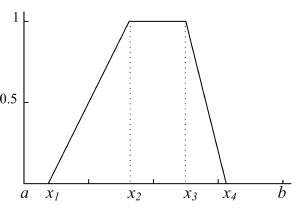
\includegraphics[scale=0.8]{fig/trapese}
% 		\caption {Trapezoidal MFs}
% 		\label{fig:trapeze}
% 	\end{center}
% \end{figure}
% And a fuzzy partition with \textit{n} trapezoidal membership functions
% is defined by \textit{2n} variables ($x_{1}$,$x_{2}
% $,. .., $x_{2n} $ )(Equation \ref{eq:e1}). In this case,
% the representation is given by Figure \ref{fig:at}.

% \begin{figure}[!ht] 
% 	\begin{center}
% 		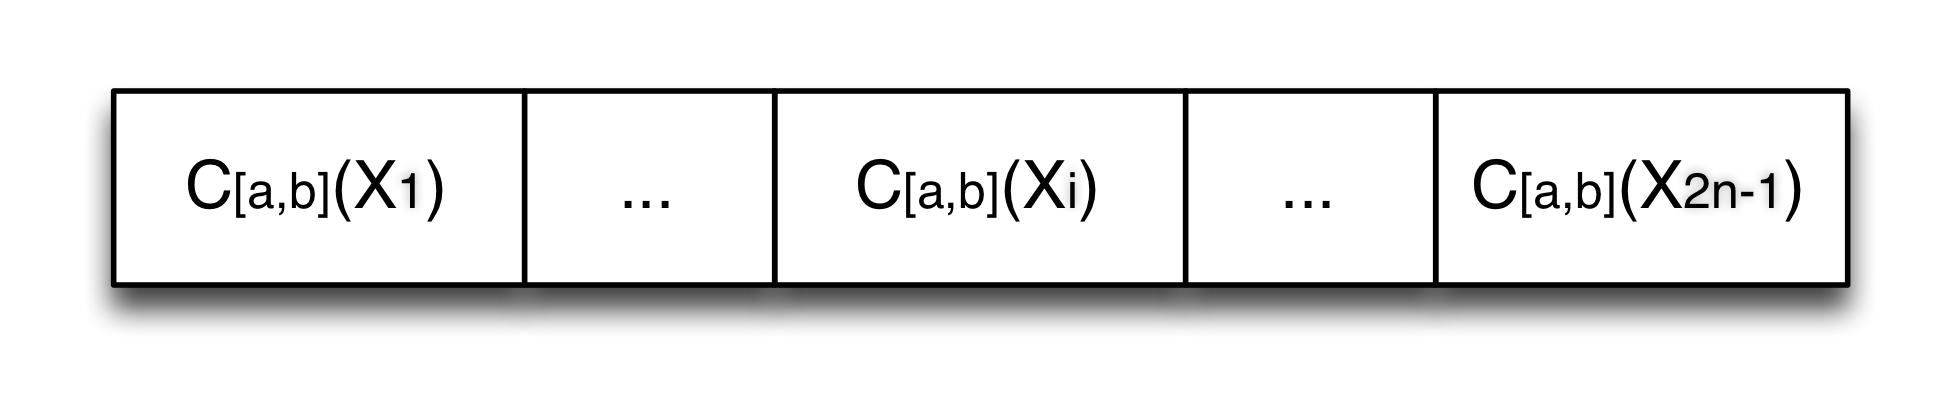
\includegraphics[scale=0.7]{fig/trapezoidal.png}
% 		\caption {Trapezoidal-shaped MFs coding}
% 		\label{fig:at}
% 	\end{center}
% \end{figure}
% With:
% \begin{equation}
% 	x_{1} \leq x_{2} \leq...\leq x_{2n-1} \leq x_{2n} 	
% \end{equation}		
% The first variable $x_{1}$ is chosen to be equal to the lower boundary of the range (\textit{a} while $x_{2n}$ is equal to \textit {b}.
% \begin{equation} 
% 	\begin{tabular}{l}
% 		$\mu_{A1}(x)=  \left \{
% 		\begin{array}{ll}
% 		1, &x_{1} \leq x \leq x_{2}\\
% 		\frac{x_{3} - x}{x_{3} - x_{2}}, &x_{2} \leq x \leq x_{3}\\
% 		0        , &x > x_{3}\\
% 		\end{array} 
% 		\right.$		\\ 	
% 		$\mu_{Ai}(x)= \left \{
% 		\begin{array}{ll} 
% 		0, &x \leq x_{2i-2}\\
% 		\frac{x - x_{2i-2}}{x_{2i-1} - x_{2i-2}}, &x_{2i-2} \leq x \leq x_{2i-1},n=2,...,i-1\\
% 		1, & x_{2i-1} \leq x \leq x_{2i}\\
% 		\frac{x_{2i+1} - x}{x_{2i+1} - x_{2i}},& x_{2i} \leq x \leq x_{2i+1}\\
% 		0  , &x > x_{2i+1}\\
% 		\end{array}  
% 		\right.	$		\\
% 		$\mu_{An}(x)= \left \{
% 		\begin{array}{ll} 
% 		0, &x \leq x_{2n-2}\\
% 		\frac{x - x_{2n-2}}{x_{2n-1} - x_{2n-2}},& x_{2n-2} \leq x \leq x_{2n-1}\\
% 		1 ,& x > x_{2n-1} 
% 		\end{array} 
% 		\right.$\\
% 		\label{eq:e1}
% 	\end{tabular}
% \end{equation}

% This is the base of the optimization conducted by the Genetic Algorithm, as it is described in the following section.


%%%%%%%%%%%%%%%%%%%%%%%%%%%%  OPTIMISING WITH GAS  %%%%%%%%%%%%%%%%%%%%%%%%%%%%

\section{Evolutionary Algorithm}
\label{sec:GA_optimization}

% ----------------------------- We need to rewrite most of this
% ---------------
% Antonio - done. I have rewritten it

As aforementioned, the proposed fuzzy sub-controllers were optimised by means of a Genetic Algorithm (GAs) \cite{GAs_Goldberg89}, aiming to find the optimal parameter values of their respective membership functions.

The followed process is shown in Figure \ref{fig:ga}. 

 \begin{figure}[!ht]
 	\label{fig:ga}
 	\begin{center}
 		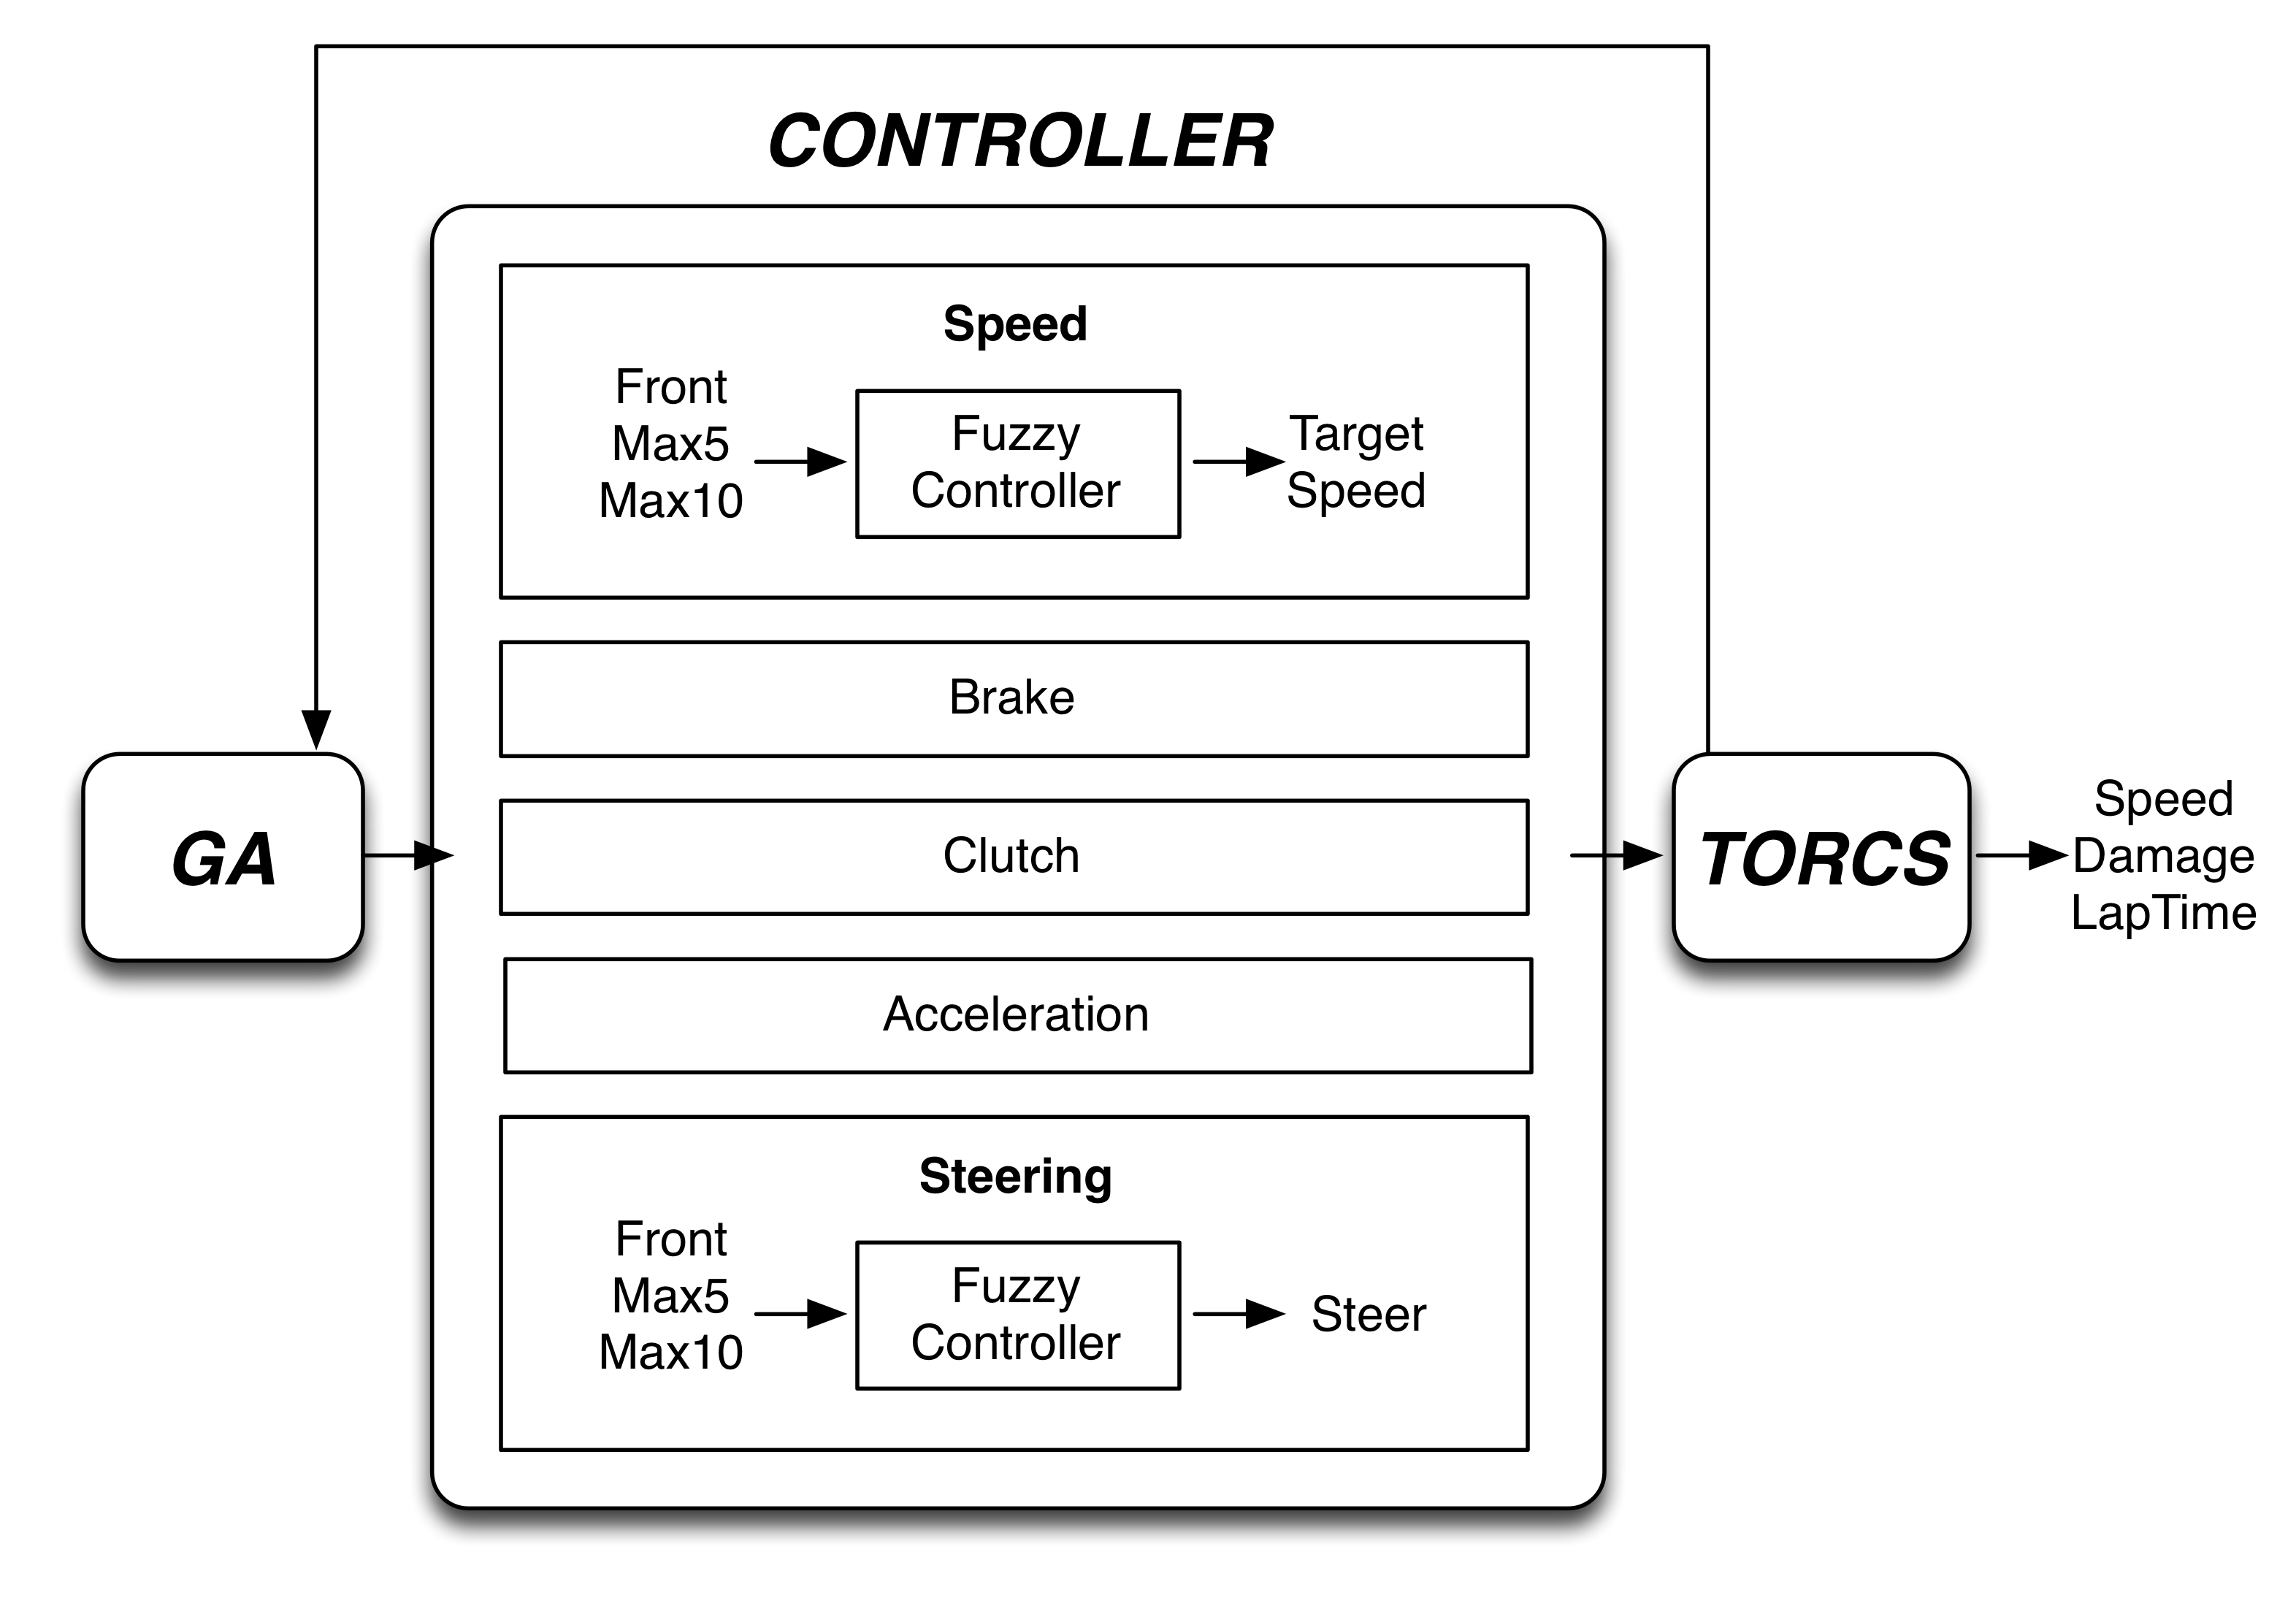
\includegraphics[width=9cm]{fig/flowchart}
 	\end{center}
 	\caption{Flowchart of the optimization process of a TORCS fuzzy controller. To evaluate an individual we put the parameter values of the two sub-controllers in the corresponding chromosome, then we launch a race in TORCS with this configuration, obtaining the resulting values of Average Speed and Damage. Individual's fitness value is computed using these values.}
 \end{figure}

In our approach, every individual or chromosome is a vector of 18 values/parameters, 6 per variable (see Figure \ref {fig:cromosome}), coded using real values aiming to have some precision \cite{elsayed13}.

 \begin{figure*}[!ht]	
 	\begin{center}
 		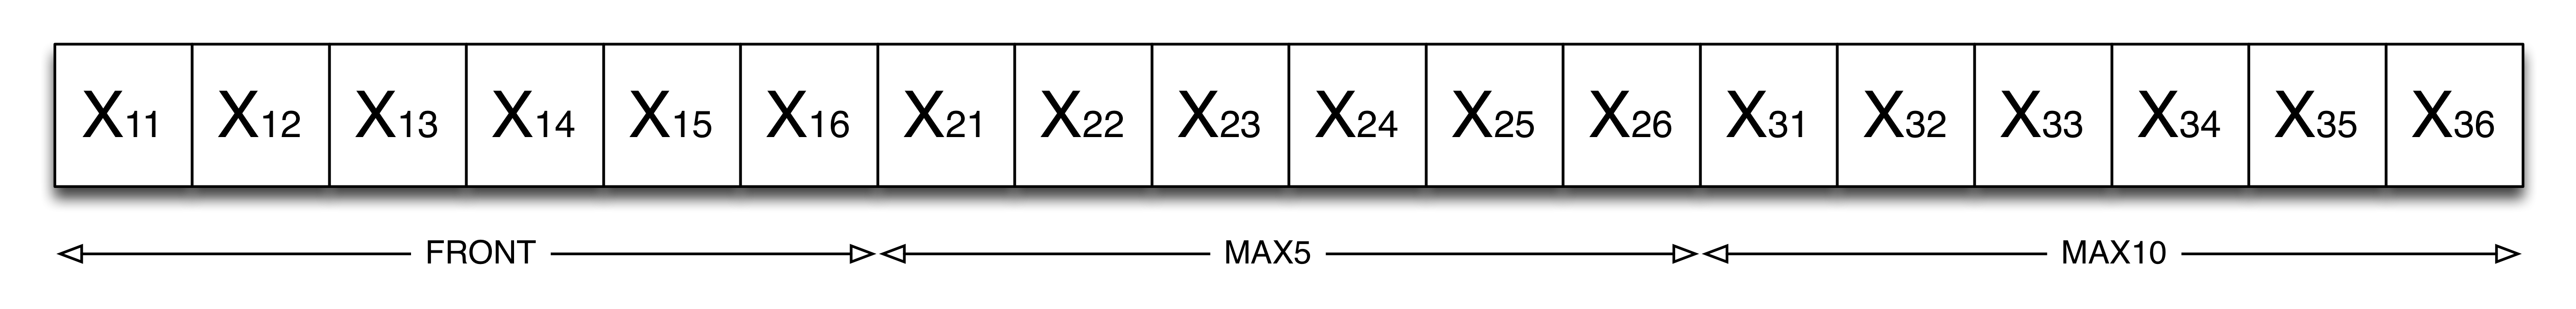
\includegraphics[width=10cm]{fig/chromosome2.png}
 		\caption{Chromosome description}
 		\label{fig:cromosome}	
 	\end{center}	
 \end{figure*}

Following standard implementations \cite{GAs_Goldberg89}, in the first step of the algorithm \cite{salem_evo17} a population of random individuals is composed by assigning diverse values inside a feasible range ($[0,100]$).

As it can be seen in Figure \ref{fig:ga}, TORCS is used for the evaluation of every individual. This evaluation is based on different fitness functions, which we have tested in previous works \cite{salem_evo18}. 
However, in this study we will consider the function which obtained the best results in our previous paper \cite{salem_cig2018}, namely:

 \begin{equation} \label{fit2}
 	\begin{array}{lll}
 		f_{AVS}= \frac{AVG(Speed)}{Damage+1}
 	\end{array}
 \end{equation}	

Following the usual recommendations in the literature \cite{Harik-ParameterLess99}, we have defined a parameter-less function, where there are no weights in the terms.
At the same time, this fitness expression is closer to a `human-like' approach, given that it is focused on the real objectives for a driver during a race, rather than on the overall target of winning or not. 

It depends on two variables:

 \begin{itemize}
 	\item $AVG(Speed)$: pursues a combination of good driving in the difficult zones of the tracks (e.g. curves) and also on easy or straight parts; i.e. considers the overall behavior in the whole track.
 	\item $Damage$: aims to create `safe' controllers, as it is mandatory being able to finish the race.
 \end{itemize} 

So the function aims to obtain drivers reaching the highest average speed as possible on the whole track while avoiding damage to the vehicle.

As it is shown in Figure \ref{fig:ga}, the fitness of each candidate solution (individual) is computed by injecting its gene values to the parameters of the membership functions of the two fuzzy sub-controllers. Then, the defined autonomous controller drives a car in a 20 laps race in a circuit without opponents, and the obtained results (Average Speed and Damage) are used to compute the fitness value. 
Given that the objective of the car controller is to win as many races as
possible, we decided to optimize the most general case by carrying out solo {\em training races}, which will be less sensitive to the presence of \textit{noise/uncertainty} due to the participation of other controllers \cite{merelo2016statistical}.

In addition, we have considered the same track as in previous works \cite{salem_cig2018} for this evaluation, because it has a proper combination of curves and straight parts. This will aid to obtain an `all-terrain behaviour' for the controllers.

Regarding the genetic operators, \textit{mutation} has remained the same as in previous approaches of our genetic controller, i.e. \textbf{non uniform mutation} \cite{mutation1997}. 

% We need to summarize this and refer to previous papers
% -------------------------

% Antonio - I have rewritten all this part. 
% Moreover, according to the invitation, this paper must be an extended version of the one published at CoG 2019, and I think it should contain a complete description of the main parts, as the Genetic algorithm proposed. I personally hate papers where you have to move to another 3 papers in order to understand the contents.


% Besides, this is also in the other paper - JJ ----------------------

% Antonio - Again, this must be an extended version and this is the main contribution. It should be here. I rewrite this.

This paper proposes the inclusion of two different mechanisms into the algorithm in order to improve its performance, as well as it allows to obtain better controllers overall.

The first technique is a \textbf{Grand Prix Selection policy} (GPS), which aims to select more reliable individuals/controllers to be parents of the following population, i.e. better deal with the uncertainty surrounding the election of an actual good individual. The mechanism arranges groups of 10 controllers (using the same car) and then different races of several laps are simulated in the same track of TORCS. After every race, the contenders obtain different scores depending on their position in the final rank. The best 5 controllers in the sum of all the races are selected as parents for the following generation. 

As it can be noticed, the application of this approach will be independent of the fitness value, so it can be considered as a \textit{fitness-less proposal}.
Thanks to this mechanism the best individuals will be more likely selected to reproduce. Of course, it is not possible to assure they are absolutely the best, due to the uncertainty present in this type of environments, i.e. games against non-deterministic opponents \cite{merelo2016statistical}. However, we argue that this selection policy will be `less sensitive' to that uncertainty (or noise), and thus, it will be fairer and more reliable than an approach purely based on the fitness values. 

On the other hand, the application of this method consumes much higher computation time, so it could be combined with the classical fitness-based selection in some generations. Indeed, in the experiments conducted in Section \ref{sec:results}, we have analysed the impact of the application of different configurations of GPS, considering a different number of generations where to apply it.

The second technique implemented in our GA is the \textbf{BLX-$\alpha$ Crossover operator} \cite{blx2008}, which allows to control the balance between exploration and exploitation along the generations.

The Blend crossover operator starts by choosing randomly a number from the interval $[x_i-\alpha(y_i-x_i).. y_i+\alpha(y_i-x_i)]$, where $x_i$ and $y_i$ are the $i^{th}$ parameter values of the parent solutions $x$,$y$ and $x_i < y_i$. See Figure \ref{fig:blxalpha}.

 \begin{figure}[!ht]	
 	\begin{center}
 		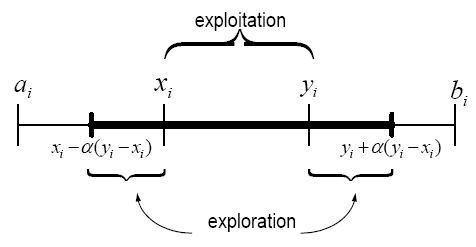
\includegraphics[width=5cm]{fig/blxalpha.jpg}
 		\caption{Blend crossover operator ($BLX-\alpha$)}
 		\label{fig:blxalpha}	
 	\end{center}	
 \end{figure}

Thus, this operator is based on the random generation of genes from the associated neighborhood of the genes in the parents. Three generated descendants are different among them and also among them and their parents, leading to a higher exploration factor in the generation of the offspring.
This operator is suitable for real coded genetic algorithms where it has proved to achieve a good balance between exploration and exploitation \cite{blx2008}.

$\alpha$ parameter allows to control the exploration of the space of solutions, depending on its value. So, in order to ensure the balance between exploitation and exploration of the search space, $\alpha = 0.5$ could be selected.

In GAs, the search process needs a high exploration rate in the first generations (high diversity) in order to explore multiple parts of the search space. But in the last generations, high exploitation is preferred to ensure the convergence to the optimal solution.

Given this, we have considered two different approaches in the experiments: one taking a constant value for $\alpha$, and another with a variable scheme, in which the value of $\alpha$ is decreased over the generations (getting sequentially more exploitation and less exploration). Thus, its value is obtained as:

 \begin{equation}
 	\label{eqalpha}
 	\alpha =1-\frac{g}{g_{max}}
 \end{equation}

Where $g$ is the current generation and $g_{max}$ is the maximum number of generations. We think that this approach can achieve an effective balance between exploitation and exploration and therefore, better solutions (better controllers) may be obtained.

% All this is also from the other paper and does not really correspond
% to what we are doing in this paper - JJ
% Antonio - Yes, we have done the same here, but extending the experiments with other configurations for the GPS. ;)

%%%%%%%%%%%%%%%%%%%%%%%%%%%%  RESULTS  %%%%%%%%%%%%%%%%%%%%%%%%%%%%

\section{Experiments and results}  
\label{sec:results}

% >>>>>> TODO: Explain the new experiments and results -> Mohammed  <<<<<<<<<<
% TODO: Results with GPS (no BLX-Alpha crossover)
% TODO: Results with GPS and BLX-Alpha crossover
% TODO: Comparison against the standard controllers in TORCS
% TODO: Comparison against S&PL controller (of all our controllers, if possible)

On the basis of the results of our previous paper \cite{salem_cig2018}, the selection of an appropriate track for training is an important factor in order to obtain competitive bots. \textit{Alpine 2} circuit has been selected for the experiments, since it combines multiple turns with straight parts (See Figure \ref{fig:alpine2_track}).

\begin{figure}[!ht]	
	\begin{center}
		
\includegraphics[width=6cm]{fig/alpine2.jpg}
		\caption{Alpine 2 Track: Slow mountain road. Length: 3773.57m, Width: 10m}
		\label{fig:alpine2_track}	
	\end{center}	
\end{figure}

As in our others studies, we have used the vehicle \textit{car1-tbr1} for our controllers, since it has a moderate performance, which will lead our controller to be prepared to drive in the most usual conditions.

New Grand Prix Selection has been conducted considering \textit{Alpine 2} track, 5 races and 20 laps per race. 
We have defined a score function based in Formula 1 Grand prix schema, so the obtained punctuations depend on the car position in the final rank: 1 - 25 points, 2 - 18, 3 - 15, 4 - 12, 5 - 10, 6 - 8, 7 - 6, 8 - 4, 9 - 2, 10 - 1. The the starting grid (initial positions of cars) on these races was set randomly.\\

To analyze the influence of the new introduced Grand Prix Selection (GPS) and the crossover operator on the performance of the fuzzy controller, we have carried out  two main optimization processes based on the GPS: the first one uses the GPS with the two point crossover operator while the second uses the varying $BLX-\alpha$. \\
In the generations where the GPS is not used, the controllers are evaluated using the fitness function: $f_{AVS}$ (Equation \ref{fit2}).
We have run the algorithms with a population size of 60 individuals. The rest of parameters are: Generations=50, Crossover rate=0.85, Mutation rate=0.09, and 10 different runs per configuration.

In each process, three experimentations are achieved, the GPS is applied in every generation in the first experimentation, only in the last generation the second and each 5 generations in the last one.
 
When Grand Prix selection process is applied as in previous work \cite{salem_cig2018}, the individuals of the population compete in 5 races (of 5 laps) in the \textit{Alpine 2} track. The last 10 individuals  in the GPS selection are replaced with new ones in the next generation. The winner will be selected as the best controller of the run.

The evolution process was applied in separate bunches of runs to obtain the following controllers:
\begin{itemize}
	\item $GFC-GPS5$: A controller obtained by applying the classical two points crossover operator (as in previous works) and GPS once every 5 generations and fitness $f_{AVS}$ in the others. 
	\item $GFC-GPSL$: A controller obtained by applying the classical two points crossover operator (as in previous works) and GPS once in the last generation and fitness $f_{AVS}$ in the others. 
	\item $GFC-GPSE$: A controller obtained by applying the classical two points crossover operator (as in previous works) and GPS every generation. 
	 
	\item $GFC-GPSVAL$: A controller obtained by applying $BLX-\alpha$ crossover operator with a varying value of $\alpha$ using Equation \ref{eqalpha} and GPS once in the last generation and fitness $f_{AVS}$ in the others. 
	 
	\item $GFC-GPSVA5$: A controller obtained by applying $BLX-\alpha$ crossover operator with a varying value of $\alpha$ using Equation \ref{eqalpha} and GPS once every 5 generations and fitness $f_{AVS}$ in the others. 
	 
	\item $GFC-GPSVAE$: A controller obtained by applying $BLX-\alpha$ crossover operator with a varying value of $\alpha$ using Equation \ref{eqalpha} and GPS every generation. 
	
		\item $GFC$: Controller  from our previous work \cite{salem_cig2018} with fitness  $f_{AVS}$ (Equation \ref{fit2}).
	\item $GFC-VA$: A controller obtained by applying $BLX-\alpha$ crossover operator with a varying value of $\alpha$ using Equation \ref{eqalpha} and fitness $f_{AVS}$. 	
\end{itemize}

Once the 10 runs have finished, the obtained best controllers from the previous evolution processes compete again in a similar set of races, in order to choose the best controller overall per approach, i.e. the best between $GFC-GPSL$, $GFC-GPSE$ and $GFC-GPS5$, and between $GFC-GPSVAL$,$GFC-GPSVAE$ and $GFC-GPSVA5$.
Results are shown in Tables\ref{tab:RSresults} and \ref{tab:VaryingalphaRSresults}
%% Process 1 : GPS without Alpha
%% Process 2  : GPS with Alpha
%%  GFC and VA are used only in comparaison purpose

\begin{table*}[ht]
	\centering
	{\scriptsize
		\caption{ Results of $GFC-GPS$ controllers in a mini-championship with 10 drivers and 10
			races in two different tracks(20 laps each). {\tt tita}, {\tt berniw} and {\tt
				inferno} are example controllers included with the TORCS
			simulator \cite{torcs4}. We use {\bf boldface}
                      for the best value, {\em italics} for the second
                    best. }
		{
			\begin{tabular}{|c|c|c||c|}
				\hline
				Driver&Score in \textit{Alpine 2} track &Score in \textit{E-Track 5} track &Total\\
				\hline
				\hline
				
			$GFC-GPS5$&	75	&74&	149\\
			$GFC-GPSE$&	98	&93&	{\bf 191}\\
			$GFC-GPSL$&	77	&81&	{\em 158}\\
			$GFC$	&	56	&50&	106\\
			$GFC-VA$	&	46	&7&		53\\
			$inferno1$&	9	&8&		17\\
			$inferno2$&		20	&51&	71\\
			$berniw1$&	16	&24&	40\\
			$berniw2$&	76	&79&	155\\
			$tita1$&32	&38&	70\\		
				\hline
				
			\end{tabular}
		}\label{tab:RSresults}
	}
\end{table*}
%


%
\begin{table*}[ht]
	\centering
	{\scriptsize
		\caption{ Results of $GFC-VAGPS$ controllers in a mini-championship with 10 drivers and 10
			races in two different tracks(20 laps each). {\tt tita}, {\tt berniw} and {\tt
				inferno} are example controllers included with the TORCS
			simulator \cite{torcs4}. {\bf Boldface}
                      for the absolute winner, {\em italics} for the second
                    best.}
		{
			\begin{tabular}{|c|c|c||c|}
				\hline
				Driver&Score in \textit{Alpine 2} track &Score in \textit{E-Track 5} track &Total\\
				\hline
				\hline	
				$GFC-VAGPS5$&	82&	82&	{\em 164}\\
				$GFC-VAGPSE$&	108&    101&	{\bf 209}\\
				$GFC-VAGPSL$&	77&	73&	150\\
				$GFC$&	56&	50&	106\\
				$GFC-VA$&	46&	7&	53\\
				$inferno1$&	9&	8&	17\\
				$inferno2$&	20&	49&	69\\
				$berniw1$&	16&	24&	40\\
				$berniw2$&	59&	73&	132\\
				$tita1$&	32&	38&	70\\			
				\hline
				
			\end{tabular}
		}\label{tab:VaryingalphaRSresults}
	}
\end{table*}
%
As it could be noticed in the Table \ref{tab:RSresults}, the controller $GFC-VGPSAE$ has win the Grand Prix championship obtaining 98 points from 125 in the track used in the training, it has also ranked first in the track  \textit{E-Track 5}. //
The other GPS based controllers have obtained nearly the same results (149 and 158 respectively).
From Table \ref{tab:RSresults},it is clear that the controller $GFC-VAGPSE$, where GPS selection has been applied in every generation, has won the majority of possible points in the two previous tracks even the unknown \textit{E-Track 5}  track.

These results come to confirm the influence of the proposed selection policy where the controllers obtained from applying the GPS selection alone have won the competition.
 
This results is evident when comparing the points obtained by GPS controllers and GFC.
Indeed, we have made the selection process  realistic by eliminating the classical fitness function based on the speed and damage average and replacing it by points obtained in direct races.//
Better speed in solo racing is not a criterion of a good driver, the best is the one who wins races. The new selection policy allows you to select the winners on the field and not the possible winners..//
The following experimentation is dedicated to detect the impact of the $BLX-\alpha$.
The best controllers obtained from the two main optimization processes: $GFC-VAGPSE$ and $GFC-GPSE$ are evaluated in formula like championship against the references five TORCS bots and the $GFC-VA$ and $GFC$ controllers. We have considered also an opponent from the state of the art, which participated in several Simulated Car Racing Competitions in past editions. 
It was proposed by P{\'e}rez-Li{\'e}bana, S{\'a}ez, Recio and Isasi \cite{EvolvingRuleSystem08} and later refined in the work \cite{PerezEvolvingFuzzy09}. We have baptised it as PSRI in honor of its authors' surnames.Results are in Table \ref{tab:allsresults}
%
\begin{table*}[ht]
	\centering
	{\scriptsize
		\caption{ Results of $GFC-GPSVAE$ and $GFC-GPSE$ controller in a mini-championship with 10 drivers and 10
			races in two different tracks(20 laps each). {\tt tita}, {\tt berniw} and {\tt
				inferno} are example controllers included with the TORCS
			simulator \cite{torcs4}.  {\bf Boldface} is
                        used to highlight the best value, {\em italics} for the second
                    best.}
		{
			\begin{tabular}{|c|c|c||c|}
				\hline
				Driver&Score in \textit{Alpine 2} track &Score in \textit{E-Track 5} track &Total\\
				\hline
				\hline
$GFC-GPSE$&	85&	82&	{\em 167}\\
$GFC-VAGPSE$&111&101&            {\bf 212}\\
$GFC$&		48&	55&	103\\
$PSRI$&		53&	48&	101\\
$GFC-VA$&	78&	64&	142\\
$inferno1$&	9&	8&	17\\
$inferno2$&	20&	40&	60\\
$berniw1$&	16&	24&	40\\
$berniw2$&	59&	69&	128\\
$tita1$&	26&	18&	44\\
					\hline
				
			\end{tabular}
		}\label{tab:allsresults}
	}
\end{table*}
%



The above competition clearly demonstrates the superiority of the $GFC-VAGPSE$ controller where it clearly leads in the points. It collected most of the points in the two tracks, leaving the $GFC-GPSE$ controller far behind it. The reference conductors, namely $GFC-VA$ and $GFC$  are classified 3rd and 5th.
The introduction of the $BLX-\alpha$ operator allows the parameters of the controllers to be refined and  increases diversification in the optimization process, which has led to better results than those of $GFC-GPSE$.

To evaluate the cost of the proposed controllers, the table \ref{tab:time} shows the average number of laps % Isn't this
% average running time? - JJ
%% each lap in Alpine 2  takes between 90s and 120s
%%  I prefered the laps number to high time values ( 123800s for instance) 
and the range of the generation where the best individual is found of all the considered controllers. These results are obtained by running genetic
optimization for 50 generations for 10 runs.  

\begin{table}[!ht]
	\centering
	{\scriptsize
          \caption{Average number of laps per generation %  Isn't this
                                %  average running time? - JJ
            and
                  generation where the best individual was spawned.}
		\label{tab:time}
		\begin{tabular}{|p{2.85cm}|p{1.65cm}|p{1.65cm}|}
			\hline 	
			\hline  
			Controller& \textbf{Average Runtime}&\textbf{Generation}\\					
			\hline \textbf{\textbf{$GFC$}}&296 &34-39\\
			\hline \textbf{$GFC-VA$}&298	&10-18\\	
			\hline \textbf{$GFC-GPSL$}& 322&23-38\\	
			\hline \textbf{$GFC-GPS5$}&689	&24-38\\	
			\hline \textbf{$GFC-GPSE$}&	2488&22-40\\	
			\hline \textbf{$GFC-VAGPSL$}&321	&9-15\\	
			\hline\textbf{$GFC-VAGPS5$}&	691&8-17\\	
			\hline\textbf{$GFC-VAGPSE$}&2489	&11-18\\					
			\hline 
		\end{tabular}
		
	}
\end{table} 

The two $GFC-VAGPSE$ and $GFC-GPSE$ controllers were the best where they are ranked 1st and 2nd but they are very expensive in runtime where they have performed around 2490 laps in Alpine 2, which is a huge learning time.
The proposed selection policy is effective but in return requires a lot of time.

Another point that we can highlight is that the controllers with $BLX-\alpha$ have reach the optimal solution in few generations (between the 10th and the 20th) while the other methods required more generations


%%TODO upload  the results of skewness and kurtosis of the evolution expermientations

An analysis study of the distribution  of the genetic individuals of three evolution processes $GFC$, $GFC-GPSE$ and $GFC-VAGPS5$.
The skewness and kurtosis are computed for $20\%$ chosen randomly fitness values after the first, the 20th and the last generation for the three controllers (See Figure \ref{fig:gfcsk},\ref{fig:gfcrsesk} and Figure \ref{fig:gfcvarsesk})


\begin{figure}[!ht]	
	\begin{center}
		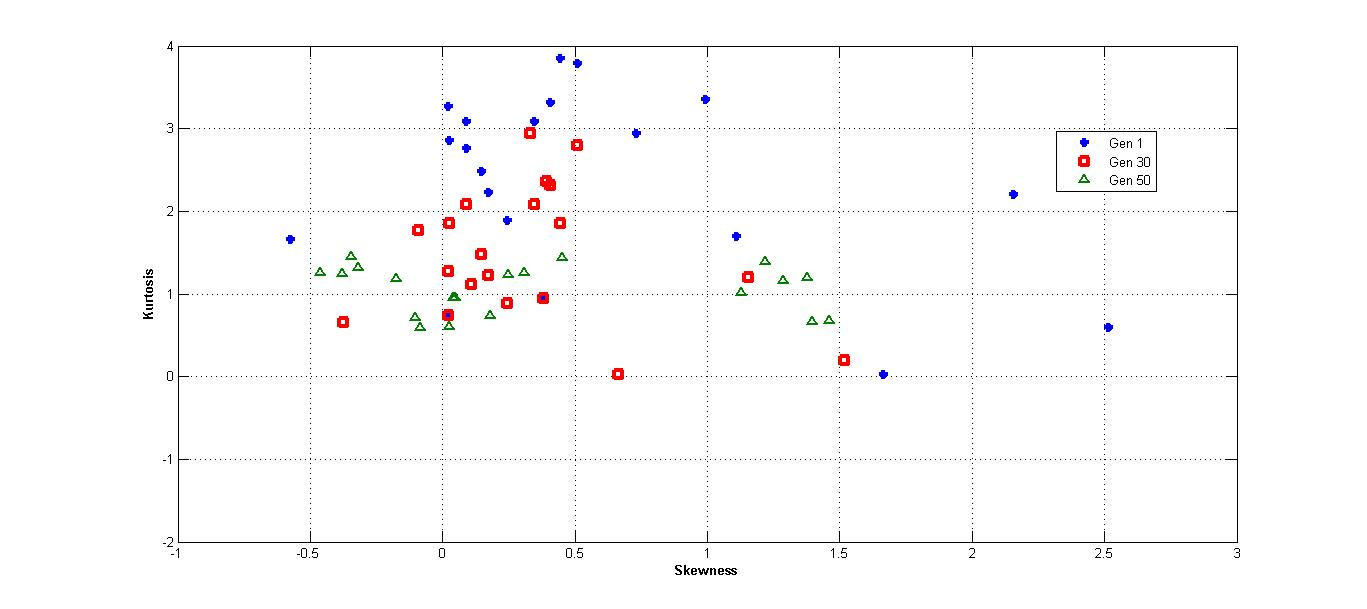
\includegraphics[width=10cm]{fig/gfc.jpg}
		\caption{Skewness and kurtosis for fitness in several generations
			of the  $GFC$}
		\label{fig:gfcsk}	
	\end{center}	
\end{figure}
\begin{figure}[!ht]	
	\begin{center}
		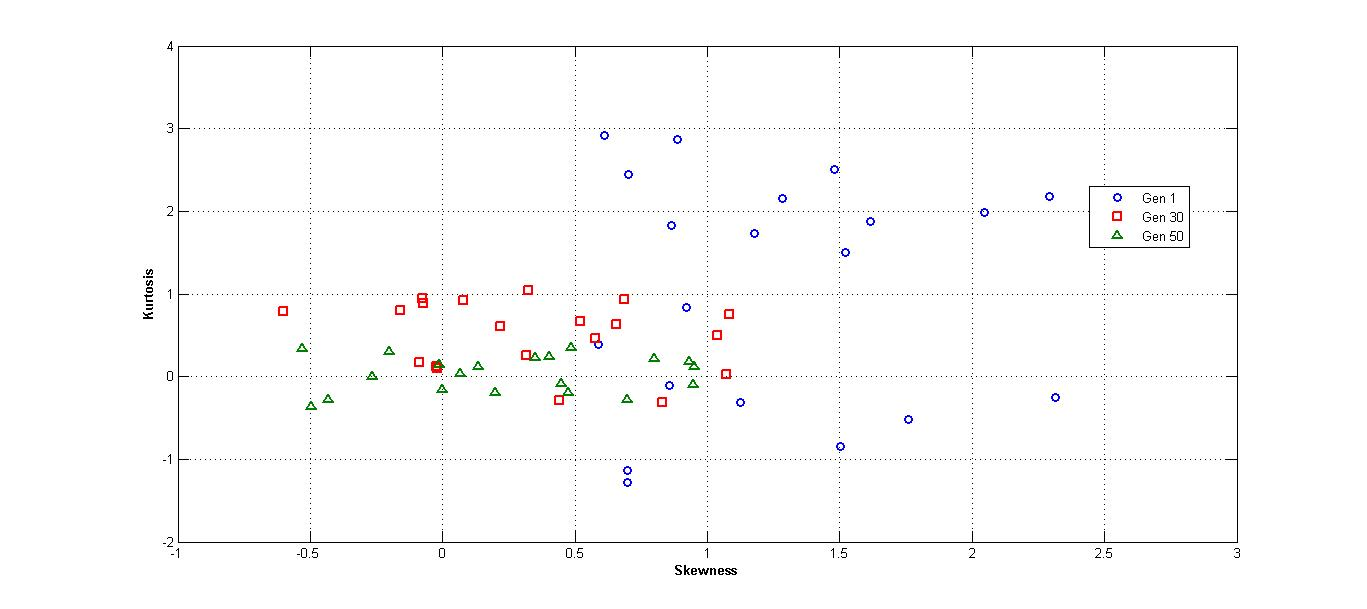
\includegraphics[width=10cm]{fig/gfcrse.jpg}
		\caption{Skewness and kurtosis for fitness in several generations
			of the  $GFC-GPSE$}
		\label{fig:gfcrsesk}	
	\end{center}	
\end{figure}
\begin{figure}[!ht]	
	\begin{center}
		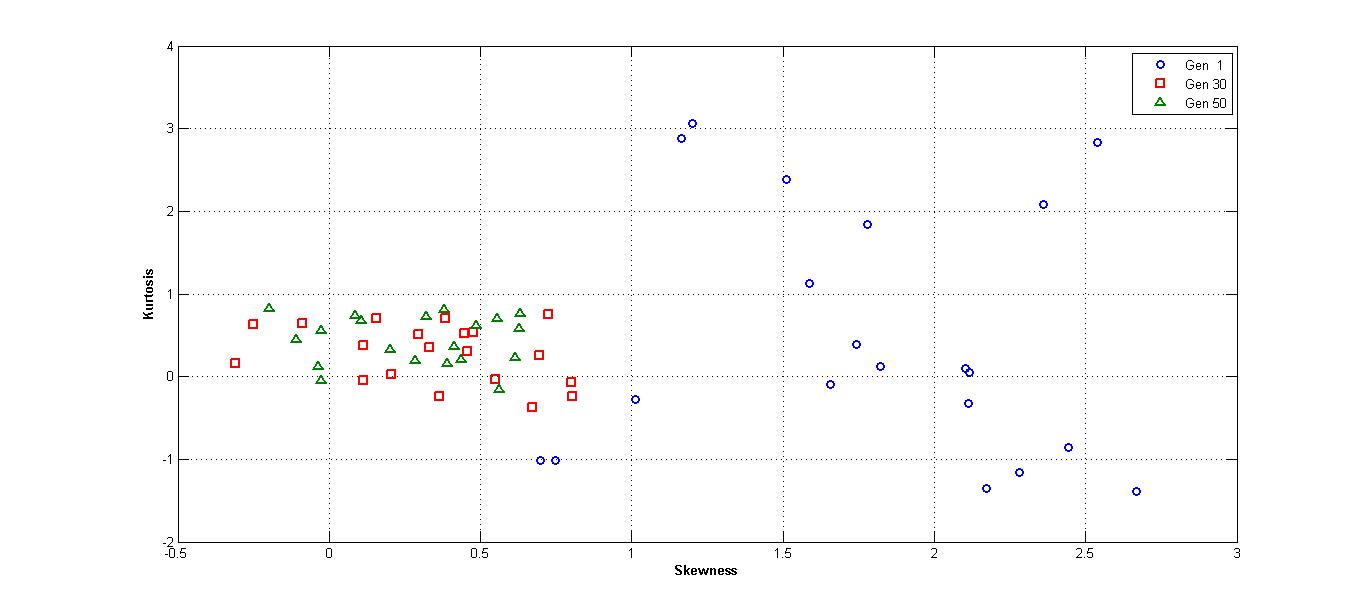
\includegraphics[width=10cm]{fig/gfcvarse.jpg}
		\caption{Skewness and kurtosis for fitness in several generations
			of the  $GFC-VAGPSE$}
		\label{fig:gfcvarsesk}	
	\end{center}	
\end{figure}

When comparing the three figures, a clear convergence, 
is observed as generations pass but without reaching, the normal distribution; in the first
generations, values of skewness and kurtosis are quite
high and correspond to arbitrary uniform distribution, however, as the simulation proceeds, values
approach zero. However, they do not converge
exactly to 0, meaning that, even if uncertainty can be
approached by a normal distribution, that approximation
would only be correct for the latest generations\cite{noisylunch2015}.
Another remarkable fact is the faster the convergence is in the case of $GFC-VAGPSE$ where it reaches its optimal values around the 20th generation to confirm the results of Table \ref{tab:time} where this controller evolution process has given the best individual between the eleventh and the eighteenth generation.
This convergence speed is the result of the combination of $Alpha-BLX$ operator and the GPS which highly pressure the chromosomes.

 %%%%%%%%%%%%%%%%%%%%%%%%%%%%
\section{Conclusions and Future Work} 
\label{sec:conclusions}

% >>>>>> TODO: Rewrite this section -> All  <<<<<<<<<<


% In this paper we have tried to get winning racing car drivers by
% first improving the selection process so that, from time to time,
% uncertainty is eliminated by using actual competitions instead of
% fitness-based evolution, and second, keep the balance between
% exploration and exploitation high, and also variable, by using a fixed
% and adaptive version of the BLX-$\alpha$ operator.

% The fuzzy genetic controller is subject to uncertainties in the track especially in case of presence of rivals so in order to overcome this problem and thus design a robust and reliable bot, we proposed to apply a \textit{Grand Prix Selection policy} where the selection of parents in the evolutionary process is carried out according to the results of a set of mini-championships organized among the individuals of the population, which looks like a car racing tournament selection.
% At the same time, and aiming to intensify the exploration process in the search space, we used the $BLX-\alpha$ crossover operator with decreasing values of the $\alpha$ parameter throughout the generations.

% The evaluation was performed by comparing the proposed controller with bots of the TORCS platform, yielding very good results.
% The other evaluation of our controller was a confrontation with a real bot ($PSRI$ controller), which participated in several Simulated Car Racing Competitions. In this case, the BLX operator and the new selection policy have had a lot of impact in helping our controller to win three quarters of the races by getting the lowest damage, average speed and maximum speed values.

% These results let us to think that our controller could have reached a very good rank in the Simulated Car Racing Competition, which is unfortunately over since 2013. Anyway, we think that the findings of this study (and previous ones) could be applied successfully to other car racing simulators, such as those used in current eSports Competitions, such as iRace (https://www.iracing.com/).

% As future lines of work, this controller can be improved in some ways:
% We can extend the selection policy to all generations while overcoming the computation time drawback by means of a parallel implementation.
% We can also explore other parameter-less fitness functions to evaluate individuals including other factors affecting the performance of the car.
% Another perspective is to use multiple tracks (instead of just one) in the selection process in order to train a more general controller, able to deal with many different situations.

\section*{Acknowledgments}

This work has been supported in part by: Ministerio espa\~{n}ol de
Econom\'{\i}a y Competitividad under projects  TIN2017-85727-C4-2-P (UGR-DeepBio) and TEC2015-68752 (also funded by FEDER).

\bibliographystyle{IEEEtranS}
\bibliography{fuzzy_torcs,geneura,uncertainty}



\begin{IEEEbiographynophoto}{Juan~J.~Merelo}
Biography text here.
\end{IEEEbiographynophoto}

% You can push biographies down or up by placing
% a \vfill before or after them. The appropriate
% use of \vfill depends on what kind of text is
% on the last page and whether or not the columns
% are being equalized.

%\vfill

% Can be used to pull up biographies so that the bottom of the last one
% is flush with the other column.
%\enlargethispage{-5in}



% that's all folks
\end{document}


